%   File: Golfer.tex
% Author: Adam Leeper
%------------------------------------------------------------------------------
%\\[0.45pc]
\providecommand{\isolatedBuild}[1]{#1}% Fallback definition to build normally.
\isolatedBuild{
  \documentclass[11pt,letterpaper]{book}
  %\documentclass[11pt,letterpaper]{book}

% aleeper: I think these are needed for Paul's macros?
\usepackage{epsfig}
\usepackage{epstopdf}

%\makeatletter
%\typeout{The import path is \import@path}
%\makeatother

\usepackage{import}

\subimport{./}{packagesMitiguy.sty}
\subimport{./}{macrosMitiguy.tex}
\subimport{./}{PageStylesMitiguy.tex}
\subimport{./}{macrosLeeper.tex}
   % Found via TEXINPUTS environment variable.
  \isolatedBuildHeader{Projectile Motion Examples}
                      {Projectile Motion of a Golf Ball
    %\footnote{Answer: With $v_o = 80 ft/s at \degrees{45}, d = 166 ft.
    %Adapted from exercise 12-102, Engineering Mechanics Dynamics,
    %R.C. Hibbeler, 12th ed., Pearson, 2010.}
    %\footnote{Answer: With $v_o = 20 ft/s at \degrees{60}, t = ??? sec.
    %Adapted from exercise 12-102, Engineering Mechanics Dynamics,
    %R.C. Hibbeler, 12th ed., Pearson, 2010.}
  }
}
%%%
%%%
%%%
{
\small
\begin{minipage}{0.50\textwidth}
  A golf ball, $Q$, is struck with an initial velocity of 20 m/s in the
  direction shown by the arrow.
  Let the earth be a Newtonian frame, \basis{N}, and assume the gravitational
  constant is $g = 9.81$ m/s$^2$.
  Neglecting air resistance, we can model the forces on the ball as
  $\force{Q} \equals -mg~\uvecy{n}$.
\end{minipage}
\hfill
\begin{minipage}{0.43\textwidth}
  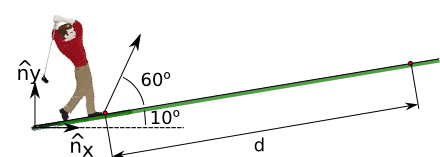
\includegraphics[width=\linewidth]{golfer.png}
\end{minipage}
%
\\[0.5pc]
\begin{itemize}
  \item Introduce appropriate measures to describe the kinematics of the ball.
  \item Use Newton's law to \textbf{show} how to get a pair of \textbf{scalar}
    differential equations describing the ball's motion.
  \item Determine the \textbf{time} that the ball is in the air.
\end{itemize}
}
\isolatedBuildFooter
